
%%% Local Variables: 
%%% mode: latex
%%% TeX-master: t
%%% End: 

% 20131021 Home 11:33
% Begin the draft writing, hope everything is safe and sound.
% Always be self-motivating.

% 20131021 Home 13:45
% Will continue my work an hour later. As with no table in the
% lab, it's really a tough situation. @OpenLab. Holycow...

% 20131021 Home 19:30
% Let's finish half of this.

% 20131024 Home 8:30
% For the former days, I do not even have the time and/or energy
% to do the update of this......Modification time. In Linux, it's
% called "mtime".

% 20131024 Home 17:10
% Almost finished my part. A few more paragraphs of "More Related Work"
% can be added. But not today. The rest of the day will go to, Data Mining
% homework, Information Security homework, Software Engineering feature development.
% As with SE, some python course will be viewed. Okay, let's solve the Windows
% problem. ---->After that, Data Mining homework time.

% 20131031 Home 00:00
% You have to do something. That's how you grow.
% It is not hard. It is hard because you do not work hard.
% Could you please use the up-to-date and more prestigious
% papers......

% 20131128 Lab 18:00
% Born in Nepal is just a joke. (Could you please not chit chat right
% now? It is still the working hours. I have some research work to
% do. See those fucking people.) So proud as a Chinese. Well, flesh
% batteries. 

% 20131129 Lab 20:40
% What I earn is all by the hardwork.







%% bare_jrnl.tex
%% V1.3
%% 2007/01/11
%% by Michael Shell
%% see http://www.michaelshell.org/
%% for current contact information.
%%
%% This is a skeleton file demonstrating the use of IEEEtran.cls
%% (requires IEEEtran.cls version 1.7 or later) with an IEEE journal paper.
%%
%% Support sites:
%% http://www.michaelshell.org/tex/ieeetran/
%% http://www.ctan.org/tex-archive/macros/latex/contrib/IEEEtran/
%% and
%% http://www.ieee.org/



% *** Authors should verify (and, if needed, correct) their LaTeX system  ***
% *** with the testflow diagnostic prior to trusting their LaTeX platform ***
% *** with production work. IEEE's font choices can trigger bugs that do  ***
% *** not appear when using other class files.                            ***
% The testflow support page is at:
% http://www.michaelshell.org/tex/testflow/


%%*************************************************************************
%% Legal Notice:
%% This code is offered as-is without any warranty either expressed or
%% implied; without even the implied warranty of MERCHANTABILITY or
%% FITNESS FOR A PARTICULAR PURPOSE!
%% User assumes all risk.
%% In no event shall IEEE or any contributor to this code be liable for
%% any damages or losses, including, but not limited to, incidental,
%% consequential, or any other damages, resulting from the use or misuse
%% of any information contained here.
%%
%% All comments are the opinions of their respective authors and are not
%% necessarily endorsed by the IEEE.
%%
%% This work is distributed under the LaTeX Project Public License (LPPL)
%% ( http://www.latex-project.org/ ) version 1.3, and may be freely used,
%% distributed and modified. A copy of the LPPL, version 1.3, is included
%% in the base LaTeX documentation of all distributions of LaTeX released
%% 2003/12/01 or later.
%% Retain all contribution notices and credits.
%% ** Modified files should be clearly indicated as such, including  **
%% ** renaming them and changing author support contact information. **
%%
%% File list of work: IEEEtran.cls, IEEEtran_HOWTO.pdf, bare_adv.tex,
%%                    bare_conf.tex, bare_jrnl.tex, bare_jrnl_compsoc.tex
%%*************************************************************************

% Note that the a4paper option is mainly intended so that authors in
% countries using A4 can easily print to A4 and see how their papers will
% look in print - the typesetting of the document will not typically be
% affected with changes in paper size (but the bottom and side margins will).
% Use the testflow package mentioned above to verify correct handling of
% both paper sizes by the user's LaTeX system.
%
% Also note that the "draftcls" or "draftclsnofoot", not "draft", option
% should be used if it is desired that the figures are to be displayed in
% draft mode.
%
\documentclass[journal]{IEEEtran}
%
% If IEEEtran.cls has not been installed into the LaTeX system files,
% manually specify the path to it like:
% \documentclass[journal]{../sty/IEEEtran}





% Some very useful LaTeX packages include:
% (uncomment the ones you want to load)


% *** MISC UTILITY PACKAGES ***
%
%\usepackage{ifpdf}
% Heiko Oberdiek's ifpdf.sty is very useful if you need conditional
% compilation based on whether the output is pdf or dvi.
% usage:
% \ifpdf
%   % pdf code
% \else
%   % dvi code
% \fi
% The latest version of ifpdf.sty can be obtained from:
% http://www.ctan.org/tex-archive/macros/latex/contrib/oberdiek/
% Also, note that IEEEtran.cls V1.7 and later provides a builtin
% \ifCLASSINFOpdf conditional that works the same way.
% When switching from latex to pdflatex and vice-versa, the compiler may
% have to be run twice to clear warning/error messages.






% *** CITATION PACKAGES ***
%
\usepackage[noadjust]{cite}
% cite.sty was written by Donald Arseneau
% V1.6 and later of IEEEtran pre-defines the format of the cite.sty package
% \cite{} output to follow that of IEEE. Loading the cite package will
% result in citation numbers being automatically sorted and properly
% "compressed/ranged". e.g., [1], [9], [2], [7], [5], [6] without using
% cite.sty will become [1], [2], [5]--[7], [9] using cite.sty. cite.sty's
% \cite will automatically add leading space, if needed. Use cite.sty's
% noadjust option (cite.sty V3.8 and later) if you want to turn this off.
% cite.sty is already installed on most LaTeX systems. Be sure and use
% version 4.0 (2003-05-27) and later if using hyperref.sty. cite.sty does
% not currently provide for hyperlinked citations.
% The latest version can be obtained at:
% http://www.ctan.org/tex-archive/macros/latex/contrib/cite/
% The documentation is contained in the cite.sty file itself.






% *** GRAPHICS RELATED PACKAGES ***
%
\ifCLASSINFOpdf
  \usepackage[pdftex]{graphicx}
  % declare the path(s) where your graphic files are
  \graphicspath{{Figure/}{../pdf/}{../jpeg/}}
  % and their extensions so you won't have to specify these with
  % every instance of \includegraphics
  \DeclareGraphicsExtensions{.pdf,.jpeg,.png}
\else
  % or other class option (dvipsone, dvipdf, if not using dvips). graphicx
  % will default to the driver specified in the system graphics.cfg if no
  % driver is specified.
  \usepackage[dvips]{graphicx}
  % declare the path(s) where your graphic files are
  \graphicspath{{Figure/}{../eps/}}
  % and their extensions so you won't have to specify these with
  % every instance of \includegraphics
  \DeclareGraphicsExtensions{.eps}
\fi
% graphicx was written by David Carlisle and Sebastian Rahtz. It is
% required if you want graphics, photos, etc. graphicx.sty is already
% installed on most LaTeX systems. The latest version and documentation can
% be obtained at:
% http://www.ctan.org/tex-archive/macros/latex/required/graphics/
% Another good source of documentation is "Using Imported Graphics in
% LaTeX2e" by Keith Reckdahl which can be found as epslatex.ps or
% epslatex.pdf at: http://www.ctan.org/tex-archive/info/
%
% latex, and pdflatex in dvi mode, support graphics in encapsulated
% postscript (.eps) format. pdflatex in pdf mode supports graphics
% in .pdf, .jpeg, .png and .mps (metapost) formats. Users should ensure
% that all non-photo figures use a vector format (.eps, .pdf, .mps) and
% not a bitmapped formats (.jpeg, .png). IEEE frowns on bitmapped formats
% which can result in "jaggedy"/blurry rendering of lines and letters as
% well as large increases in file sizes.
%
% You can find documentation about the pdfTeX application at:
% http://www.tug.org/applications/pdftex





% *** MATH PACKAGES ***
%
\usepackage[cmex10]{amsmath}
% A popular package from the American Mathematical Society that provides
% many useful and powerful commands for dealing with mathematics. If using
% it, be sure to load this package with the cmex10 option to ensure that
% only type 1 fonts will utilized at all point sizes. Without this option,
% it is possible that some math symbols, particularly those within
% footnotes, will be rendered in bitmap form which will result in a
% document that can not be IEEE Xplore compliant!
%
% Also, note that the amsmath package sets \interdisplaylinepenalty to 10000
% thus preventing page breaks from occurring within multiline equations. Use:
\interdisplaylinepenalty=2500
% after loading amsmath to restore such page breaks as IEEEtran.cls normally
% does. amsmath.sty is already installed on most LaTeX systems. The latest
% version and documentation can be obtained at:
% http://www.ctan.org/tex-archive/macros/latex/required/amslatex/math/





% *** SPECIALIZED LIST PACKAGES ***
%
\usepackage{algorithmic}
% algorithmic.sty was written by Peter Williams and Rogerio Brito.
% This package provides an algorithmic environment for describing algorithms.
% You can use the algorithmic environment in-text or within a figure
% environment to provide for a floating algorithm. Do NOT use the algorithm
% floating environment provided by algorithm.sty (by the same authors) or
% algorithm2e.sty (by Christophe Fiorio) as IEEE does not use dedicated
% algorithm float types and packages that provide these will not provide
% correct IEEE style captions. The latest version and documentation of
% algorithmic.sty can be obtained at:
% http://www.ctan.org/tex-archive/macros/latex/contrib/algorithms/
% There is also a support site at:
% http://algorithms.berlios.de/index.html
% Also of interest may be the (relatively newer and more customizable)
% algorithmicx.sty package by Szasz Janos:
% http://www.ctan.org/tex-archive/macros/latex/contrib/algorithmicx/




% *** ALIGNMENT PACKAGES ***
%
\usepackage{array}
% Frank Mittelbach's and David Carlisle's array.sty patches and improves
% the standard LaTeX2e array and tabular environments to provide better
% appearance and additional user controls. As the default LaTeX2e table
% generation code is lacking to the point of almost being broken with
% respect to the quality of the end results, all users are strongly
% advised to use an enhanced (at the very least that provided by array.sty)
% set of table tools. array.sty is already installed on most systems. The
% latest version and documentation can be obtained at:
% http://www.ctan.org/tex-archive/macros/latex/required/tools/


\usepackage{mdwmath}
\usepackage{mdwtab}

% Also highly recommended is Mark Wooding's extremely powerful MDW tools,
% especially mdwmath.sty and mdwtab.sty which are used to format equations
% and tables, respectively. The MDWtools set is already installed on most
% LaTeX systems. The lastest version and documentation is available at:
% http://www.ctan.org/tex-archive/macros/latex/contrib/mdwtools/


% IEEEtran contains the IEEEeqnarray family of commands that can be used to
% generate multiline equations as well as matrices, tables, etc., of high
% quality.


\usepackage{eqparbox}
% Also of notable interest is Scott Pakin's eqparbox package for creating
% (automatically sized) equal width boxes - aka "natural width parboxes".
% Available at:
% http://www.ctan.org/tex-archive/macros/latex/contrib/eqparbox/





% *** SUBFIGURE PACKAGES ***
%\usepackage[tight,footnotesize]{subfigure}
% subfigure.sty was written by Steven Douglas Cochran. This package makes it
% easy to put subfigures in your figures. e.g., "Figure 1a and 1b". For IEEE
% work, it is a good idea to load it with the tight package option to reduce
% the amount of white space around the subfigures. subfigure.sty is already
% installed on most LaTeX systems. The latest version and documentation can
% be obtained at:
% http://www.ctan.org/tex-archive/obsolete/macros/latex/contrib/subfigure/
% subfigure.sty has been superceeded by subfig.sty.



%\usepackage[caption=false]{caption}
%\usepackage[font=footnotesize]{subfig}
% subfig.sty, also written by Steven Douglas Cochran, is the modern
% replacement for subfigure.sty. However, subfig.sty requires and
% automatically loads Axel Sommerfeldt's caption.sty which will override
% IEEEtran.cls handling of captions and this will result in nonIEEE style
% figure/table captions. To prevent this problem, be sure and preload
% caption.sty with its "caption=false" package option. This is will preserve
% IEEEtran.cls handing of captions. Version 1.3 (2005/06/28) and later
% (recommended due to many improvements over 1.2) of subfig.sty supports
% the caption=false option directly:
\usepackage[caption=false,font=footnotesize]{subfig}
%
% The latest version and documentation can be obtained at:
% http://www.ctan.org/tex-archive/macros/latex/contrib/subfig/
% The latest version and documentation of caption.sty can be obtained at:
% http://www.ctan.org/tex-archive/macros/latex/contrib/caption/




% *** FLOAT PACKAGES ***
%
\usepackage{fixltx2e}
% fixltx2e, the successor to the earlier fix2col.sty, was written by
% Frank Mittelbach and David Carlisle. This package corrects a few problems
% in the LaTeX2e kernel, the most notable of which is that in current
% LaTeX2e releases, the ordering of single and double column floats is not
% guaranteed to be preserved. Thus, an unpatched LaTeX2e can allow a
% single column figure to be placed prior to an earlier double column
% figure. The latest version and documentation can be found at:
% http://www.ctan.org/tex-archive/macros/latex/base/



%\usepackage{stfloats}
% stfloats.sty was written by Sigitas Tolusis. This package gives LaTeX2e
% the ability to do double column floats at the bottom of the page as well
% as the top. (e.g., "\begin{figure*}[!b]" is not normally possible in
% LaTeX2e). It also provides a command:
%\fnbelowfloat
% to enable the placement of footnotes below bottom floats (the standard
% LaTeX2e kernel puts them above bottom floats). This is an invasive package
% which rewrites many portions of the LaTeX2e float routines. It may not work
% with other packages that modify the LaTeX2e float routines. The latest
% version and documentation can be obtained at:
% http://www.ctan.org/tex-archive/macros/latex/contrib/sttools/
% Documentation is contained in the stfloats.sty comments as well as in the
% presfull.pdf file. Do not use the stfloats baselinefloat ability as IEEE
% does not allow \baselineskip to stretch. Authors submitting work to the
% IEEE should note that IEEE rarely uses double column equations and
% that authors should try to avoid such use. Do not be tempted to use the
% cuted.sty or midfloat.sty packages (also by Sigitas Tolusis) as IEEE does
% not format its papers in such ways.


%\ifCLASSOPTIONcaptionsoff
%  \usepackage[nomarkers]{endfloat}
% \let\MYoriglatexcaption\caption
% \renewcommand{\caption}[2][\relax]{\MYoriglatexcaption[#2]{#2}}
%\fi
% endfloat.sty was written by James Darrell McCauley and Jeff Goldberg.
% This package may be useful when used in conjunction with IEEEtran.cls'
% captionsoff option. Some IEEE journals/societies require that submissions
% have lists of figures/tables at the end of the paper and that
% figures/tables without any captions are placed on a page by themselves at
% the end of the document. If needed, the draftcls IEEEtran class option or
% \CLASSINPUTbaselinestretch interface can be used to increase the line
% spacing as well. Be sure and use the nomarkers option of endfloat to
% prevent endfloat from "marking" where the figures would have been placed
% in the text. The two hack lines of code above are a slight modification of
% that suggested by in the endfloat docs (section 8.3.1) to ensure that
% the full captions always appear in the list of figures/tables - even if
% the user used the short optional argument of \caption[]{}.
% IEEE papers do not typically make use of \caption[]'s optional argument,
% so this should not be an issue. A similar trick can be used to disable
% captions of packages such as subfig.sty that lack options to turn off
% the subcaptions:
% For subfig.sty:
% \let\MYorigsubfloat\subfloat
% \renewcommand{\subfloat}[2][\relax]{\MYorigsubfloat[]{#2}}
% For subfigure.sty:
% \let\MYorigsubfigure\subfigure
% \renewcommand{\subfigure}[2][\relax]{\MYorigsubfigure[]{#2}}
% However, the above trick will not work if both optional arguments of
% the \subfloat/subfig command are used. Furthermore, there needs to be a
% description of each subfigure *somewhere* and endfloat does not add
% subfigure captions to its list of figures. Thus, the best approach is to
% avoid the use of subfigure captions (many IEEE journals avoid them anyway)
% and instead reference/explain all the subfigures within the main caption.
% The latest version of endfloat.sty and its documentation can obtained at:
% http://www.ctan.org/tex-archive/macros/latex/contrib/endfloat/
%
% The IEEEtran \ifCLASSOPTIONcaptionsoff conditional can also be used
% later in the document, say, to conditionally put the References on a
% page by themselves.





% *** PDF, URL AND HYPERLINK PACKAGES ***
%
\usepackage{url}
% url.sty was written by Donald Arseneau. It provides better support for
% handling and breaking URLs. url.sty is already installed on most LaTeX
% systems. The latest version can be obtained at:
% http://www.ctan.org/tex-archive/macros/latex/contrib/misc/
% Read the url.sty source comments for usage information. Basically,
% \url{my_url_here}.


% Some personal house keeping
\usepackage{booktabs}
\usepackage{hyperref}
\hypersetup{unicode}
\hypersetup{colorlinks=true}
\hypersetup{linkcolor=black}





% *** Do not adjust lengths that control margins, column widths, etc. ***
% *** Do not use packages that alter fonts (such as pslatex).         ***
% There should be no need to do such things with IEEEtran.cls V1.6 and later.
% (Unless specifically asked to do so by the journal or conference you plan
% to submit to, of course. )


% correct bad hyphenation here
\hyphenation{op-tical net-works semi-conduc-tor}


\begin{document}
%
% paper title
% can use linebreaks \\ within to get better formatting as desired
%\title{Bare Demo of IEEEtran.cls for Journals}

% Abraham: There will be a good title afterwards.
\title{Mining Customer Data with Ensemble Selection}

%
%
% author names and IEEE memberships
% note positions of commas and nonbreaking spaces ( ~ ) LaTeX will not break
% a structure at a ~ so this keeps an author's name from being broken across
% two lines.
% use \thanks{} to gain access to the first footnote area
% a separate \thanks must be used for each paragraph as LaTeX2e's \thanks
% was not built to handle multiple paragraphs
%

%\author{Michael~Shell,~\IEEEmembership{Member,~IEEE,}
%        John~Doe,~\IEEEmembership{Fellow,~OSA,}
%        and~Jane~Doe,~\IEEEmembership{Life~Fellow,~IEEE}% <-this % stops a space
\author{Yanan~Xiao,~\IEEEmembership{Student Member,~IEEE,}
Aziza~Al~Sawafi%
\thanks{Y. Xiao, A. Sawafi are 1st year master students with the Department of
Electrical Engineering and Computer Science, Masdar Institute of Science and Technology, Masdar City,
Abu Dhabi, UAE.\@ P.O. 54224\@ Email: \{yxiao,aalsawafi@masdar.ac.ae\}.}%
\thanks{One team member quit Masdar Institute not soon after the
  project. But we managed to get things done by ourselves.}}
%\thanks{M. Shell is with the Department
%of Electrical and Computer Engineering, Georgia Institute of Technology, Atlanta,
%GA, 30332 USA e-mail: (see http://www.michaelshell.org/contact.html).}% <-this % stops a space
%\thanks{J. Doe and J. Doe are with Anonymous University.}% <-this % stops a space
%\thanks{Manuscript received April 19, 2005; revised January 11, 2007.}}
%

% note the % following the last \IEEEmembership and also \thanks -
% these prevent an unwanted space from occurring between the last author name
% and the end of the author line. i.e., if you had this:
%
% \author{....lastname \thanks{...} \thanks{...} }
%                     ^------------^------------^----Do not want these spaces!
%
% a space would be appended to the last name and could cause every name on that
% line to be shifted left slightly. This is one of those "LaTeX things". For
% instance, "\textbf{A} \textbf{B}" will typeset as "A B" not "AB". To get
% "AB" then you have to do: "\textbf{A}\textbf{B}"
% \thanks is no different in this regard, so shield the last } of each \thanks
% that ends a line with a % and do not let a space in before the next \thanks.
% Spaces after \IEEEmembership other than the last one are OK (and needed) as
% you are supposed to have spaces between the names. For what it is worth,
% this is a minor point as most people would not even notice if the said evil
% space somehow managed to creep in.



% The paper headers
%\markboth{Journal of \LaTeX\ Class Files,~Vol.~6, No.~1, January~2007}%
%{Shell \MakeLowercase{\textit{et al.}}: Bare Demo of IEEEtran.cls for Journals}
\markboth{Journal of Masdar Institute,~Vol.~1, No.~15, December~2013}%
{Xiao \MakeLowercase{\textit{et al.}}: Data Mining Midterm Project Report}
% The only time the second header will appear is for the odd numbered pages
% after the title page when using the twoside option.
%
% *** Note that you probably will NOT want to include the author's ***
% *** name in the headers of peer review papers.                   ***
% You can use \ifCLASSOPTIONpeerreview for conditional compilation here if
% you desire.




% If you want to put a publisher's ID mark on the page you can do it like
% this:
%\IEEEpubid{0000--0000/00\$00.00~\copyright~2007 IEEE}
% Remember, if you use this you must call \IEEEpubidadjcol in the second
% column for its text to clear the IEEEpubid mark.



% use for special paper notices
%\IEEEspecialpapernotice{(Midterm Report)}




% make the title area
\maketitle


\begin{abstract}
%\boldmath
%The abstract goes here.
We present our approach to the big data problem put forward in KDD
Cup 2009. We carry out a more technical analysis of our initial plan.
And we describe our trials and errors with the large dataset. Till
now, our team has not come up with any practical solution with large
dataset in a limited time. We present our results with the small
dataset in the end.



\end{abstract}
% IEEEtran.cls defaults to using nonbold math in the Abstract.
% This preserves the distinction between vectors and scalars. However,
% if the journal you are submitting to favors bold math in the abstract,
% then you can use LaTeX's standard command \boldmath at the very start
% of the abstract to achieve this. Many IEEE journals frown on math
% in the abstract anyway.

% Note that keywords are not normally used for peerreview papers.
\begin{IEEEkeywords}
%IEEEtran, journal, \LaTeX, paper, template.
Customer relationship prediction, ensemble selection, classification,
data mining
% The keywords may be changed later if we adopt another method.
\end{IEEEkeywords}






% For peer review papers, you can put extra information on the cover
% page as needed:
% \ifCLASSOPTIONpeerreview
% \begin{center} \bfseries EDICS Category: 3-BBND \end{center}
% \fi
%
% For peerreview papers, this IEEEtran command inserts a page break and
% creates the second title. It will be ignored for other modes.
\IEEEpeerreviewmaketitle



\section{Introduction}\label{sec:introduction}
% The very first letter is a 2 line initial drop letter followed
% by the rest of the first word in caps.
%
% form to use if the first word consists of a single letter:
% \IEEEPARstart{A}{demo} file is ....
%
% form to use if you need the single drop letter followed by
% normal text (unknown if ever used by IEEE):
% \IEEEPARstart{A}{}demo file is ....
%
% Some journals put the first two words in caps:
% \IEEEPARstart{T}{his demo} file is ....
%
% Here we have the typical use of a "T" for an initial drop letter
% and "HIS" in caps to complete the first word.
%\IEEEPARstart{T}{his} demo file is intended to serve as a ``starter file''
%for IEEE journal papers produced under \LaTeX\ using
%IEEEtran.cls version 1.7 and later.
% You must have at least 2 lines in the paragraph with the drop letter
% (should never be an issue)
%I wish you the best of success.

%\hfill mds

%\hfill January 11, 2007


%\subsection{Subsection Heading Here}
%Subsection text here.

% needed in second column of first page if using \IEEEpubid
%\IEEEpubidadjcol

%\subsubsection{Subsubsection Heading Here}
%Subsubsection text here.
\IEEEPARstart{C}{ustomer} relationship management (CRM) is an
essential model for managing the interactions between the company and
its current and future customers. It takes up-to-date technologies to
organize, automate, and synchronize CRM and marketing information
system~\cite{Ref:CustomerRelationshipManagement}. CRM applications
that use data mining are called Analytic CRM, which provides valid
predictions from customer data collected and stored with various
attributes. There are a lot of data mining tools and methods to
extract and analyze data generally, and customer data specifically. A
naive step in doing so is to summarize the statistical attributes of
the data (such as means and standard deviations) and use charts and
graphs to review it
visually~\cite{Ref:DataMiningStrategiesforCRM}. However, in many
situations customer relationship data volume is vast and
massive. Therefore, more sophisticated methods are created and
evaluated. In this field, we found the following techniques are most
frequently employed: decision trees, support vector machines,
artificial neural networks and Bayesian classifiers.
\par
Data mining has powerful capability in processing and analyzing data;
its key technologies that applied in CRM are categorized into three
main categories; clustering, classification and forecast, and
association
rules~\cite{Ref:ApplicationOfDataMiningInCRM}. Classification and
forecast analysis classifies unknown data into the most proper
pre-defined class based on category description that is obtained by
training a set of data using certain algorithm. Key classification
techniques are; decision making tree, Bayesian statistics, BP neural
networks, Genetic Algorithm, rough set theory, fuzzy set theory and so
on. Classification methods in CRM can predict new customer’s behaviors
and activities. 
\par
As mentioned in~\cite{Ref:TargetingCustomers}, classification analysis
is the one that is widely used in classifying CRM data. It can be
processed in two steps; learning phase and training
phase~\cite{Ref:AnalysisOfTheKDDCup2009}. In the learning phase the
classification algorithm analyzes the training data set and learns it,
then in the second phase the accuracy of the classifier will be
estimated using the test data set. After that, the classifier can be
used to predict and classify new data set. In order to obtain better
accuracy, some preprocessing and filtering techniques can be applied
to the data before going through the classification phases. Those
techniques are; data cleaning, data discretization, and feature
selection. The common challenges in knowledge discovery from CRM data
are the high-dimensionality, and imbalanced corrupted
records. Besides, researchers roved that customer classification and
prediction is cost sensitive in nature. For example, if a valuable
customer predicted as loyal but then that customer churns, the cost is
higher than if a loyal customer is classified as one who will
churn~\cite{Ref:ChallengesinKDDataMiningDatasets}.
\par
In this paper, we present various tools that we tried and several
plans that were carried out when dealing with big data problem like
this. The rest of the paper is organized as
follows. Section~\ref{sec:initial-plan} displays what our thoughts
were before tackling the real large dataset. Section
\ref{sec:revised-proposal} shows what our efforts are when no team
member has the pre-knowledge of how to write \emph{map reduce} scripts
and run them with the help of
clusters. Section~\ref{sec:result-conclusion} serves as the conclusion
for this not-so-successful trial with big, complex data mining task.

% After downloading the data. Upload it to Amazon. And run.



\section{Initial Proposal}
\label{sec:initial-plan}
Lesson we learn from writing and reviewing this section is that
``think twice before taking actions''. We depicted a master plan in
our previous proposal~\cite{Ref:Yanan2013}. However, due to the lack
of map reduce technique, we are able to train models on a oct-core
workstation. The problem is that the training part of ensemble
selection is really memory consuming. All of the 32GB memory got used
instantly while at the same time we observe the CPU usage just above
10\%. See Fig~\ref{fig:memory-consuming}.
\begin{figure}[!t]
\centering
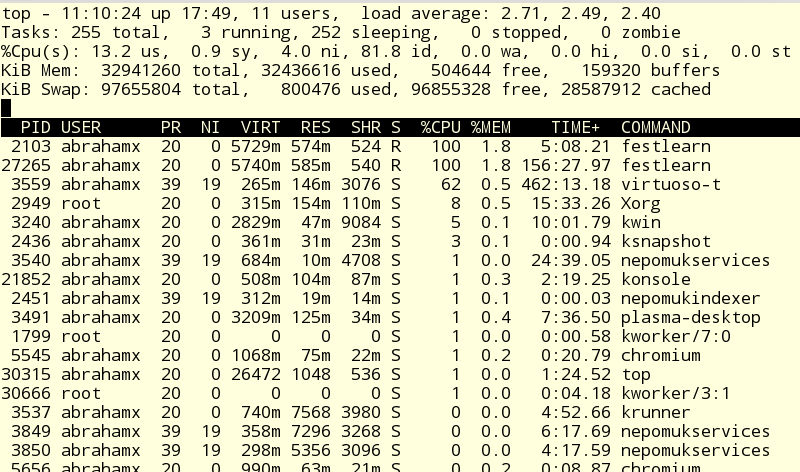
\includegraphics[scale=0.35]{Figure/Memory-Consuming.png}
% where an .eps filename suffix will be assumed under latex,
% and a .pdf suffix will be assumed for pdflatex; or what has been declared
% via \DeclareGraphicsExtensions.
\caption{CPU and memory usage when running FEST package}
\label{fig:memory-consuming}
\end{figure}

\subsection{Preprocessing}
\label{sec:preprocessing}

In order to tackle the challenges of the big data set, we propose the
following steps.
\par
Missing value. We would consider missing categorical values
as a separate value. We would take a standard approach which
calculates the mean of the feature to impute missing values. And as
proven an effective technique
by~\cite{Ref:WinningtheKDDCupIBMResearch}. We decide to add an extra
indicator variable to indicate “missingness” for every one of the 333
variables with missing values. We planned to do this because some
linear models in our base classifiers could then estimate the optimal
constant instead of merely relying on the means to replace the missing
value with. 
\par
Categorical value. Since categorical values are not easily
handled by many learning algorithms, we decide to recode categorical
values using the same way as by IBM Research. For different values a
categorical attribute could take, we would generate corresponding
indicators. As a good example shown in IBM’s paper, limiting the
number of values encoded would greatly reduce the number of features,
which may be from variables with an enormous vocabulary. 
\par
Clean up. We would normalize each feature by dividing up by their
range. And we would clean the data by eliminating redundant features,
which are either constant, or duplicate of other features.

\subsection{Base Classifiers}
\label{sec:base-classifiers}

As stated by Dietterich~\cite{Ref:EnsembleMethodsInMachineLearning},
``A necessary and sufficient condition for an ensemble of classifiers
to be more accurate than any of its individual members is if the
classifiers are accurate and diverse''. Building libraries would be
expensive, what’s more is that time is limited to train all of them in
the next phase. To maintain the accuracy and diversity of our
next-phase base classifier library, we decide to build it using the
classifiers as follows, boosted decision trees, decision trees, linear
regression, SVM and k-NN. 

\subsection{Ensemble Selection}
\label{sec:ensemble-selection}

An ensemble is a collection of models. To make predictions, we just
need to calculate weighted average or ``voting'' based on those
models. One important reason for us to work with ensemble selection is
that it can be optimized to any easily computed metric. Same as
described before, for an ensemble selection classifier used to improve
classification accuracy, one thing is the base classifiers in the
library are accurate. This is not hard to achieve with a great
literature at hand. The other characteristic is diverse. Due to the
fact that our computation power is limited, we planned to build 100 to
200 base classifiers in our library. 

\subsection{More Features and Base Classifiers}
\label{sec:more-features-base}

We planned to create some more features and base classifiers. One is
to buildup a decision tree using FEST
package~\cite{Caruana:2008:EES:1390156.1390169}, and then visualize
this tree so that we can tell distinguish a set of nodes forming the
best splitting points. We also refer to a few state-of-the-art
classifiers that claiming better performance than traditional
ones. Nevertheless, as put out in the following section, we did not
possess enough energy to handle them.

\section{Our Journey}
\label{sec:revised-proposal}
As mentioned in abstract, we are not able to produce result which
exactly follows what we depict in our midterm report. Our initiative
is to follow the step of IBM Research, which outperformed other teams
in KDD Cup 2009. We started our more detailed background investigation
right after the submission of midterm report. Our first attempt was to
set up a cluster with the help of Amazon Web
Service\footnote{\url{http://aws.amazon.com/ec2/}}. We tried several
times but were not able to make the whole cluster share a same virtual
disk, which is vital according
to~\cite{ref:ensembleselectionnutshell}. Our review on this failure is
that we should set off even earlier after being informed that this is
a real classification problem on really complex data. After the
submission, we also investigate tools like hadoop, MongoDB and Apache
Mahout\cite{NIPS2006_725}. Because the time is limited and each team
member has other research task at hand, we plan to run our initial
plan on a Amazon cluster later on. Below we discuss our process step
by step.

\subsection{MATLAB}
\label{sec:matlab}

Our preprocessing is done fairly standard and systematic. We use
MATLAB to load the plaintext feature chunk and then run pre-written
scripts to format them following the previous guidelines. A note here
is that when dealing with large datasets like this, it's also memory
consuming. The memory consumption in total for train and test chunk
sums up to 10GB.\@ We then use the built-in function \emph{csvwrite}
to format them. This is important because tools we use, like FEST
package, BBR package, and LIBSVM, only supports LIBSVM format. The
final conversion is done with a c program that helps transform csv
format files into libsvm format. This step is also done automatically
by writing a shell script.
\par
One thing that is worth noting here is that we actually did two types
of preprocessing, one pretty naive whereas the other strictly
following the standard. So for our team we have as many as two sets of
large data and two sets of small data. Our story with small data is
discussed in the next section since we finished it after the deadline,
because we really want to produce some results. For the naive
preprocessing, we merely transformed the categorical data to
numerical, and skip any other step. We later find this strategy
performed badly due to some obvious reasons: large dimensionality,
large data scale for transformed categorical data, and redundant or
even noisy feature. 
\par
After the first attempt of ``lazy'' preprocessing, the strict version
is carried out as follows:
\begin{enumerate}
\item Impute both missing numerical and categorical values with their
  mean at that column.
  \begin{itemize}
  \item If one column is composed of all $NaN$ values, it is tagged
    $1$.
  \item Else it is tagged $2$. 
  \item The value that is tagged $1$ then gets deleted because no
    information could be obtained from that feature. This treatment is
    also useful to indicate missingness. 
  \end{itemize}
\item Recode the categorical values by sorting and selecting. We
  select top 10 largest categorical events, and recode them by
  computing their frequency in the corresponding feature. If there are
  fewer than 10 events, all of them get kept and recoded. 
\item The last step we do is to normalize each feature value and then
  mapping them to scale $[-1, 1]$. 
\end{enumerate}
We also plan to carry out some classification with MATLAB built-in
function \emph{TreeBagger} later on. Since both team member agree that
following IBM's method is a good way, for the large dataset we still
try to tackle it with FEST packages and the alike.


\subsection{Weka}
\label{sec:weka}

Weka is the first integrated tool that came to our mind. The author
mentioned in the manual that even a sample of real-world data that's
processed with ensemble selection could take days or even weeks to
run\cite{ref:ensembleselectionnutshell}. There are two built-in model
libraries in weka's ensemble selection package, both are
``incredibly'' large. We follow the instructions on this manual and
describe our attempt with Weka as follows:
\begin{enumerate}
\item Build a model list with library editor GUI implemented in weka's
  ensemble selection package. One thing worth noting here is that
  since the newest stable version, EnsembleSelection package is not
  shipped as a built-in package. The model list file is actually a xml
  file containing command information to be read and executed by
  weka. 
\item The file we try with weka is in csv format. It will be
  transformed to arff format once the classification, in our case
  ensemble selection command, is entered. Part of our command is
  supplied in the appendices.
\end{enumerate}
As indicated in manual ``Ensemble Selection in a Nutshell'', training
takes time when the dimension of data is large. And this is especially
the case with KDD Cup's dataset. We deal with more than 14,000
features this time because we did not delete as many features as IBM
did. Moreover, the large dataset contains 50,000 instances. We did run
weka to get a result successfully. Training that feature requires
almost 24 hours and one model file output by the Ensemble Selection
weka implementation would take as much as 4.2GB harddisk space. Since
this is the first time that we deal with \emph{big data} using weka,
with no help from tools like hadoop to map reduce the problem, we
decided to abandon it for practical considerations, like time,
harddisk space, etc. 
\begin{figure}[!t]
  \centering
  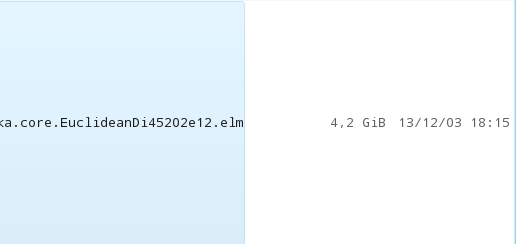
\includegraphics[scale=0.5]{Age-of-Big-Data9}
  \caption{One model file trained by Weka ensemble selection package}
  \label{fig:weka-1}
\end{figure}




 

% This part shall be finished as soon as possible. And go to bed as
% well as get up early, my friend. 

\subsection{Specific Packages}
\label{sec:specific-packages}
After the first two trials, we find that it is too resource consuming
to train and classify big data using ensemble selection method via
more generic tools like MATLAB and Weka. And that seem to explain why
IBM research team did not employ tools as such. Another interesting
thing we find is that even software like Hadoop that is built to help
distributed computing is written in Java, which appears to be the
``best practice'' for some time.
\par
We choose FEST, LIBSVM and BBR packages in the end. For FEST package
we use it to train random forest as well as boosted decision
trees. Even with the fully preprocessed data, it still takes a long
time to train \emph{one} random forest or boosted decision
tree. In~\autoref{fig:specific-packages-2} it is demonstrated how time
consuming it is when the package program was not written for parallel
purpose. And~\autoref{fig:specific-packages-3} shows the related
training time for those models. 
\begin{figure}[!t]
  \centering
  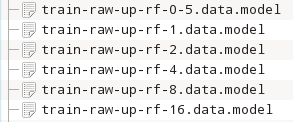
\includegraphics{Age-of-Big-Data6}
  \caption{Model files trained by FEST package}
  \label{fig:specific-packages-2}
\end{figure}

\begin{figure}[!t]
  \centering
  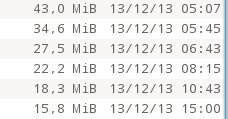
\includegraphics{Age-of-Big-Data5}
  \caption{Corresponding training time for some random forest models}
  \label{fig:specific-packages-3}
\end{figure}

The LIBSVM package~\cite{Chang:2011:LLS:1961189.1961199} is used to
train models based on support vector machine technique. We also
prepared shell scripts for this step. Unfortunately, due to the
practice in map reduce technique, even if the CPU of our workstation
has a 80\% idle rate, we can hardly run all those scripts in
parallel. The BRR package is obtained for logistic regression usage
for which we also prepared automatic shell
scripts~\cite{Genkin:August2007:0040-1706:291}.   
\par
Without the assistance from powerful map reduce tools, till now we
have trained random forest models of appetency, churn and
upselling. The classification is still on-going. We also manually run
the \emph{festclassify} program during the training process, the best
result we get is $0.991667$ as the prediction probability for one
instances. The other prediction file that we have has the distribution
as shown in~\autoref{fig:special-package-1}.
\begin{figure}[!t]
  \centering
  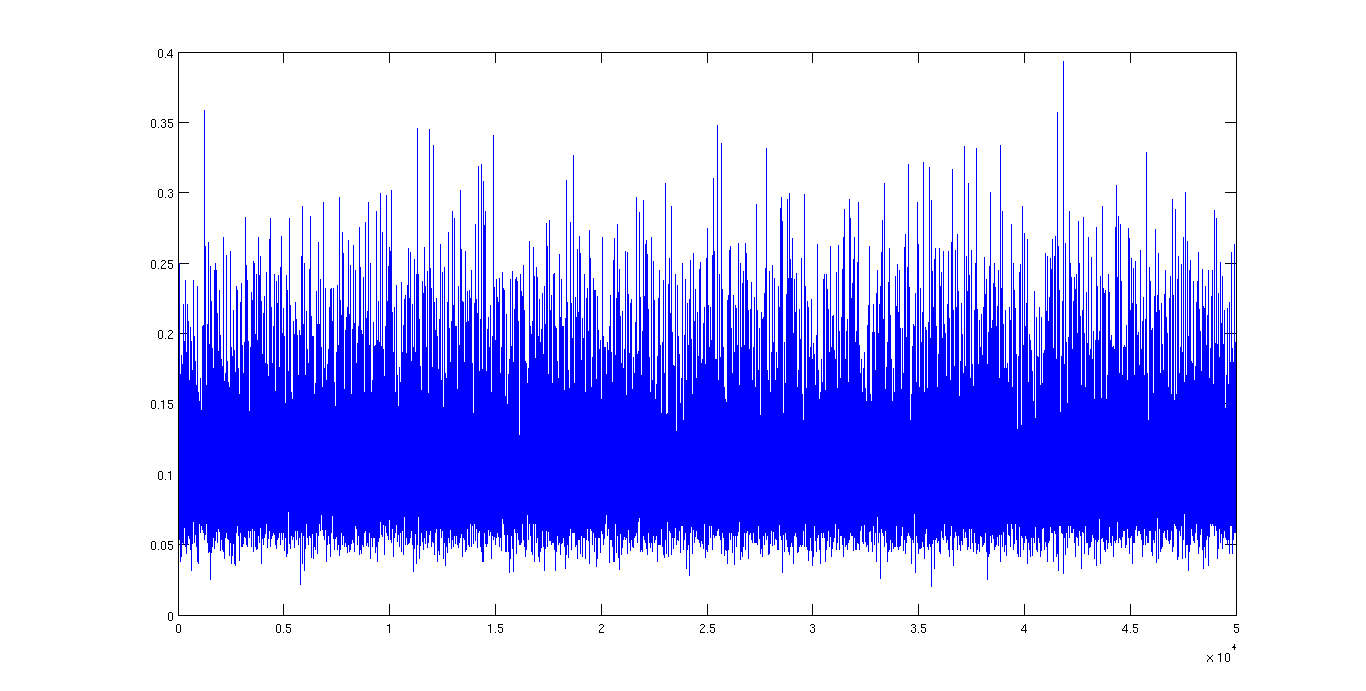
\includegraphics[scale=0.2]{train-plot}
  \caption{Prediction Distribution for One Churn Model}
  \label{fig:special-package-1}
\end{figure}
The distribution looks fine but we haven't found out any reasonable
explanation why the mean of this prediction is only $0.1034$. For the
$0.991667$ prediction, we suppose that overfitting is one possible
explanation. 

\subsection{Small Dataset}
\label{sec:small-dataset}
In addition to our original plan, we also practiced with the small
dataset the moment we find it impractical to stick with ensemble
selection. Overall ensemble selection as described
in~\cite{Caruana:2008:EES:1390156.1390169} can have good performance
on high dimension dataset, but that point stands on the basis of
carefully running either Weka program or specific packages \emph{in
  parallel}. Due to the lack of related knowledge in map reduce, we
run similar classifiers on Weka with small dataset. We describe our
results as follows.
\par
The preprocessing is carried out in a similar manner not parameters
are not 100\% the same.
\begin{enumerate}
\item If an feature contains more than 50\% missing values,
  i.e. ``NaN'' in MATLAB terminology, then this feature is no longer
  considered. 
\item For the remaining features, we impute missing values as follows:
  \begin{enumerate}
  \item Both missing values in numerical and categorical features are
    imputed with their modes and means.
  \item Categorical values are recoded to numerical values, by their
    relative frequency.
  \item For each feature the discretization is applied to smooth
    distribution curve.
  \end{enumerate}
\item The final clean up is done by filtering features that possesses
  a less than $0.01$ information gain. We use Weka's built-in function
  InfoGainAttributeEval filter to achieve this step.
\end{enumerate}
For small dataset, we also carry out the classification with two
samples of data. One set we removed categorical features completely
the other is full, for the benefit of comparison. The base classifiers
we use in this case are Naive Bayesian Classifier (NBC), Lazy IBK and
Decision Table Classifier (DTC). NBC is simple in structure and it is
based on the assumption that predictors are conditionally independent
given the target variable. Because of its simplicity, NBC was
attractive choice since we have a large set of variables.  The second
classifier is Lazy IBK (Instance-Based K) which is one of the Nearest
Neighbor algorithms. Thirdly, we used DTC which uses a simple decision
table majority algorithm; it makes decisions on attributes for each
instance.
\par
Our results with the small dataset is displayed as follows.
% \begin{table}[!t]
% %increase table row spacing, adjust to taste
% \renewcommand{\arraystretch}{1.3}
% %if using array.sty, it might be a good idea to tweak the value of
% %\extrarowheight as needed to properly center the text within the cells
% \caption{An Example of a Table}
% \label{table_example}
% \centering
% %Some packages, such as MDW tools, offer better commands for making tables
% %than the plain LaTeX2e tabular which is used here.
% \begin{tabular}{|c||c|}
% \hline
% One & Two\\
% \hline
% Three & Four\\
% \hline
% \end{tabular}
% \end{table}

\begin{table}
[!t]
\centering
\caption{Small dataset without categorical values}
\label{tab:small-dataset-1}
\begin{tabular}
{ccccc}
\toprule
Method & ~ & AUC & ~ & ~\\
~ & Churn & Appetency & Upselling & Score\\
\hline
NBC & 0.529 & 0.497 & 0.658 & 0.561\\
Lazy IBK & 0.532  & 0.525 & 0.619 & 0.558\\
DTC & 0.53 & 0.5 & 0.757 & 0.595\\
\bottomrule
\end{tabular}
\end{table}

\begin{table}
[!t]
\centering
\caption{Small dataset with full preprocessed values}
\label{tab:small-dataset-2}
\begin{tabular}
{ccccc}
\toprule
Method & ~ & AUC & ~ & ~\\
~ & Churn & Appetency & Upselling & Score\\
\hline
NBC & 0.568 & 0.523 & 0.682 & 0.591\\
Lazy IBK & 0.533  & 0.5 & 0.564 & 0.532\\
DTC & 0.53 & 0.5 & 0.756 & 0.595\\
\bottomrule
\end{tabular}
\end{table}
















\section{Results and Conclusion}
\label{sec:result-conclusion}
For the implementation of our blueprint that was discussed in our
midterm report, we, as a solid team of two, have tried our best to
obtain results using ensemble selection technique. Our results with
large dataset are far from being satisfactory and we plan to have some
discussions with course lecturer to figure out possible reasons.
\par
We set off at an early time for this final project, but neither team
member has sufficient technical background in this field to solve this
project ``safe and sound''. We are a team of two but each other did
the following things:
\begin{itemize}
\item Yanan Xiao. He tried various methods to tackle large dataset and
  wanted to stick to the team's initial plan, i.e.\ ensemble selection
  with around 300 base classifiers. He is in charge of the report
  typesetting in IEEE template with \LaTeX2e{}.
\item Aziza Al Sawafi. She came up with the small dataset workaround
  and successfully got some results. She also tried to solve this
  classification problem using MATLAB and LIBSVM.\@
\end{itemize}









%%*************************************************************************
% An example of a floating figure using the graphicx package.
% Note that \label must occur AFTER (or within) \caption.
% For figures, \caption should occur after the \includegraphics.
% Note that IEEEtran v1.7 and later has special internal code that
% is designed to preserve the operation of \label within \caption
% even when the captionsoff option is in effect. However, because
% of issues like this, it may be the safest practice to put all your
% \label just after \caption rather than within \caption{}.
%
% Reminder: the "draftcls" or "draftclsnofoot", not "draft", class
% option should be used if it is desired that the figures are to be
% displayed while in draft mode.
%
%\begin{figure}[!t]
%\centering
%\includegraphics[width=2.5in]{myfigure}
% where an .eps filename suffix will be assumed under latex,
% and a .pdf suffix will be assumed for pdflatex; or what has been declared
% via \DeclareGraphicsExtensions.
%\caption{Simulation Results}
%\label{fig_sim}
%\end{figure}

% Note that IEEE typically puts floats only at the top, even when this
% results in a large percentage of a column being occupied by floats.


% An example of a double column floating figure using two subfigures.
% (The subfig.sty package must be loaded for this to work.)
% The subfigure \label commands are set within each subfloat command, the
% \label for the overall figure must come after \caption.
% \hfil must be used as a separator to get equal spacing.
% The subfigure.sty package works much the same way, except \subfigure is
% used instead of \subfloat.
%
%\begin{figure*}[!t]
%\centerline{\subfloat[Case I]\includegraphics[width=2.5in]{subfigcase1}%
%\label{fig_first_case}}
%\hfil
%\subfloat[Case II]{\includegraphics[width=2.5in]{subfigcase2}%
%\label{fig_second_case}}}
%\caption{Simulation results}
%\label{fig_sim}
%\end{figure*}
%
% Note that often IEEE papers with subfigures do not employ subfigure
% captions (using the optional argument to \subfloat), but instead will
% reference/describe all of them (a), (b), etc., within the main caption.


% An example of a floating table. Note that, for IEEE style tables, the
% \caption command should come BEFORE the table. Table text will default to
% \footnotesize as IEEE normally uses this smaller font for tables.
% The \label must come after \caption as always.
%
%\begin{table}[!t]
%% increase table row spacing, adjust to taste
%\renewcommand{\arraystretch}{1.3}
% if using array.sty, it might be a good idea to tweak the value of
% \extrarowheight as needed to properly center the text within the cells
%\caption{An Example of a Table}
%\label{table_example}
%\centering
%% Some packages, such as MDW tools, offer better commands for making tables
%% than the plain LaTeX2e tabular which is used here.
%\begin{tabular}{|c||c|}
%\hline
%One & Two\\
%\hline
%Three & Four\\
%\hline
%\end{tabular}
%\end{table}


% Note that IEEE does not put floats in the very first column - or typically
% anywhere on the first page for that matter. Also, in-text middle ("here")
% positioning is not used. Most IEEE journals use top floats exclusively.
% Note that, LaTeX2e, unlike IEEE journals, places footnotes above bottom
% floats. This can be corrected via the \fnbelowfloat command of the
% stfloats package.

%%*************************************************************************



%\section{Conclusion}
%The conclusion goes here.





% if have a single appendix:
%\appendix[Proof of the Zonklar Equations]
% or
%\appendix  % for no appendix heading
% do not use \section anymore after \appendix, only \section*
% is possibly needed

% use appendices with more than one appendix
% then use \section to start each appendix
% you must declare a \section before using any
% \subsection or using \label (\appendices by itself
% starts a section numbered zero.)
%


\appendices
\section{Source Code}
%Appendix one text goes here.

% you can choose not to have a title for an appendix
% if you want by leaving the argument blank
%\section{}
%Appendix two text goes here.
We enlist our partial source codes here. The complete project is at
Github CIS501
repository\footnote{\url{https://github.com/ProfessorX/CIS501}}. 

\subsection{Preprocessing}
\label{sec:preprocessing-1}
\begin{verbatim}
%-----Recode--------%
Recode={};
for i=14703:14962
    value=unique(Train(:,i));
    value(value==0)=[];
    if ~isempty(value)
    value(:,2)=0;
    for j=1:size(value,1)
        value(j,2)=sum(Train(:,i)==
        value(j,1))/50000;
    end
    [~,lev]=sort(value(:,2),'descend');
    value=value(lev,:);
    if length(value)>10
    value=value(1:10,:);
    end
    end
    Recode{1,i-14702}=value;
    value1=unique(Test(:,i));
    value1(value1==0)=[];
    if ~isempty(value1)
    value1(:,2)=0;
    for j=1:size(value1,1)
        value1(j,2)=sum(Test(:,i)==
        value1(j,1))/50000;
    end
    [~,lev]=sort(value1(:,2),'descend');
    value1=value1(lev,:);
    if length(value1)>10
    value1=value1(1:10,:);
    end
    end
    Recode{2,i-14702}=value1;   
end
\end{verbatim}



\subsection{Automatic Shell Scripts for Building Models}
\label{sec:autom-shell-scripts}


\begin{verbatim}
#!/bin/bash
festlearn -c 3 -n 0.1 -p 0.5 -t 300 
train-raw-ap.data 
train-raw-ap-rf-0-5.data.model &&
festlearn -c 3 -n 0.1 -p 1 -t 300 
train-raw-ap.data 
train-raw-ap-rf-1.data.model &&
festlearn -c 3 -n 0.1 -p 2 -t 300 
train-raw-ap.data 
train-raw-ap-rf-2.data.model &&
festlearn -c 3 -n 0.1 -p 4 -t 300 
train-raw-ap.data 
train-raw-ap-rf-4.data.model &&
festlearn -c 3 -n 0.1 -p 8 -t 300 
train-raw-ap.data 
train-raw-ap-rf-8.data.model &&
festlearn -c 3 -n 0.1 -p 16 -t 300 
train-raw-ap.data 
train-raw-ap-rf-16.data.model &&
festlearn -c 3 -n 0.1 -p 32 -t 300 
train-raw-ap.data 
train-raw-ap-rf-32.data.model &&
festlearn -c 3 -n 0.1 -p 64 -t 300 
train-raw-ap.data 
train-raw-ap-rf-64.data.model &&
\end{verbatim}

% use section* for acknowledgment
\section*{Acknowledgment}


The authors would like to thank Dr.\ Wei Lee for giving high quality data mining lectures and selecting this challenging but rewarding topic as this semester's project. They would like give more gratitude to Masdar Institute for the studying and researching environment.


% Can use something like this to put references on a page
% by themselves when using endfloat and the captionsoff option.
\ifCLASSOPTIONcaptionsoff
  \newpage
\fi



% trigger a \newpage just before the given reference
% number - used to balance the columns on the last page
% adjust value as needed - may need to be readjusted if
% the document is modified later
%\IEEEtriggeratref{8}
% The "triggered" command can be changed if desired:
%\IEEEtriggercmd{\enlargethispage{-5in}}

% references section

% can use a bibliography generated by BibTeX as a .bbl file
% BibTeX documentation can be easily obtained at:
% http://www.ctan.org/tex-archive/biblio/bibtex/contrib/doc/
% The IEEEtran BibTeX style support page is at:
% http://www.michaelshell.org/tex/ieeetran/bibtex/
\bibliographystyle{IEEEtran}
% argument is your BibTeX string definitions and bibliography database(s)
%\bibliography{IEEEabrv,../bib/paper}
\bibliography{IEEEabrv,Reference}
%
% <OR> manually copy in the resultant .bbl file
% set second argument of \begin to the number of references
% (used to reserve space for the reference number labels box)
%\begin{thebibliography}{1}

%\bibitem{IEEEhowto:kopka}
%H.~Kopka and P.~W. Daly, \emph{A Guide to \LaTeX}, 3rd~ed.\hskip 1em plus
%  0.5em minus 0.4em\relax Harlow, England: Addison-Wesley, 1999.

%\end{thebibliography}

% Abraham: We choose to use BibTeX, this is much more manageable.

% biography section
%
% If you have an EPS/PDF photo (graphicx package needed) extra braces are
% needed around the contents of the optional argument to biography to prevent
% the LaTeX parser from getting confused when it sees the complicated
% \includegraphics command within an optional argument. (You could create
% your own custom macro containing the \includegraphics command to make things
% simpler here.)
%\begin{biography}[{\includegraphics[width=1in,height=1.25in,clip,keepaspectratio]{mshell}}]{Michael Shell}
% or if you just want to reserve a space for a photo:

%\begin{IEEEbiography}{Michael Shell}
%Biography text here.
%\end{IEEEbiography}

% if you will not have a photo at all:
\begin{IEEEbiographynophoto}{Yanan Xiao}
A first year master student as well as IEEE student member in CIS program, Masdar Institute. He loves programming when all the coursework is finished. When he feels tired of programming, he would read some books.
\end{IEEEbiographynophoto}

% insert where needed to balance the two columns on the last page with
% biographies
%\newpage

\begin{IEEEbiographynophoto}{Aziza Al Sawafi}
 First year Computing and Information Science student at Masdar Inst., got a bachelor degree in Network Engineering (United Arab Emirates University). Sport, drawing, designing, blogging, reading poems, photography, and riding horse/bicycle are my interests beside all things that are related to networking and computer science.
\end{IEEEbiographynophoto}

% You can push biographies down or up by placing
% a \vfill before or after them. The appropriate
% use of \vfill depends on what kind of text is
% on the last page and whether or not the columns
% are being equalized.

\vfill

% Can be used to pull up biographies so that the bottom of the last one
% is flush with the other column.
\enlargethispage{-5in}



% that's all folks
\end{document}



